\exercises

%%%%%%%%%%%%%%%%%%%%%%%%%%%%%%%%%%%%%%%%%%%%%%%%%%%%%%%%%%%%%%%%%%%%%%%%
% Constructor methods
%
\begin{exercise}{object1}
In Section~\ref{section:objects-functional-update} we implemented the three factory
functions \hbox{\lstinline/new_scale/}, \hbox{\lstinline/new_rotate/}, and \hbox{\lstinline/new_translate/} as methods,
claiming that it would avoid code duplication.  Write one of the factory functions as a normal
function (not a method).  How can you avoid code duplication?

\begin{answer}\ifanswers
Let's implement \hbox{\lstinline/new_scale/} as a normal function.

\begin{ocaml}
let new_scale sx sy =
   object
      val matrix = (sx, 0., 0., sy, 0., 0.)
      method transform (x, y) = $\cdots$
      method multiply matrix2 = $\cdots$
   end;;
\end{ocaml}
%
If the other functions were implemented the same way, the code for the methods \hbox{\lstinline/transform/}
and \hbox{\lstinline/multiply/} would be duplicated.  We can avoid this by creating a generic constructor
function that takes the entire matrix as an argument.

\begin{ocaml}
let new_transform matrix =
   object
      val matrix = matrix
      method transform (x, y) = $\cdots$
      method multiply matrix2 = $\cdots$
   end

let new_scale sx sy = new_matrix (sx, 0., 0., sy, 0., 0.)
let new_translate dx dy = new_matrix (1., 0., dx, 0., 1., dy)
let new_rotate theta =
   let s, c = sin theta, cos theta in
   new_transform (c, -.s, 0., s, c, 0.)
\end{ocaml}
\fi\end{answer}
\end{exercise}

%%%%%%%%%%%%%%%%%%%%%%%%%%%%%%%%%%%%%%%%%%%%%%%%%%%%%%%%%%%%%%%%%%%%%%%%
% Silly field definitions
%
\begin{exercise}{object2}
In Section~\ref{section:objects-factories} the factory functions include some apparently silly field
definitions.  For example, the function \hbox{\lstinline/new_poly/} includes the field
\hbox{\lstinline/val vertices = vertices/}.
What is the purpose of the field definition?  What would happen if it were
omitted?

\begin{answer}\ifanswers
The purpose of the code is to allow the functional update
\hbox{\lstinline/{< vertices = Array.map matrix#transform vertices >}/};
for this to work, \hbox{\lstinline/vertices/} must be a field of the object.
If the field definition were omitted, the functional update would fail.
\fi\end{answer}
\end{exercise}

%%%%%%%%%%%%%%%%%%%%%%%%%%%%%%%%%%%%%%%%%%%%%%%%%%%%%%%%%%%%%%%%%%%%%%%%
% Uniqueness
%
\begin{exercise}{object4}
Suppose we wish to enforce the fact that a program contains only one copy of an object.  For
example, the object may be an accounting object, and we wish to make sure the object is never copied
or forged.

The standard library module \hbox{\lstinline/Oo/} contains a function that copies any object.

\begin{ocaml}
   val copy : (< .. > as 'a) -> 'a
\end{ocaml}
%
Modify the following object so that it refuses to work after being copied.

\begin{ocaml}
let my_account =
object
   val mutable balance = 100
   method withdraw =
      if balance = 0 then
         raise (Failure "account is empty");
      balance <- balance - 1
end
\end{ocaml}

\begin{answer}\ifanswers
  The object is initially created with a reference \lstinline/self1/ to itself, using the \lstinline/self/ parameter,
  and the value of \lstinline/self/ is checked (with pointer equality) before the withdraw operation
  is allowed.  The value for \lstinline/self1/ has to be set in an initializer (when the value of \lstinline/self/ is known).
  For simplicity, we use the empty object \lstinline/object end/ for the initial value of \lstinline/self1/.
\begin{ocaml}
let my_account =
object (self : 'self)
    val mutable balance = 100
    val mutable self1 : < > = object end
    initializer self1 <- (self :> < >)
    method withdraw =
        if (self :> < >) != self1 then
           raise (Failure "object has been copied");
        if balance = 0 then
           raise (Failure "account is empty");
        balance <- balance - 1
end
\end{ocaml}
\fi\end{answer}
\end{exercise}

%%%%%%%%%%%%%%%%%%%%%%%%%%%%%%%%%%%%%%%%%%%%%%%%%%%%%%%%%%%%%%%%%%%%%%%%
% Subtyping
%
\begin{exercise}{classes-subtype1}
For each of the following instances of types $t_1$ and $t_2$,
determine whether $t_1$ is a subtype of $t_2$---that is, whether $t_1 \subtype t_2$.
Assume the following class declarations and relations.

\begin{center}
\begin{tabular}{|l|}
\hline
Subtyping relations\\
\hline
\hbox{\lstinline/dog $\subtype$ animal/}\\
\hbox{\lstinline/cat $\subtype$ animal/}\\
\hline
\end{tabular}
\end{center}

\begin{enumerate}
\item

\begin{ocamllisting}
type $t_1$ = animal -> cat
type $t_2$ = dog -> animal
\end{ocamllisting}

\item

\begin{ocamllisting}
type $t_1$ = animal ref
type $t_2$ = cat ref
\end{ocamllisting}

\item

\begin{ocamllisting}
type 'a cl = < f : 'a -> 'a >
type $t_1$ = dog cl
type $t_2$ = animal cl
\end{ocamllisting}

\item

\begin{ocamllisting}
type 'a cl = < x : 'a ref >
type $t_1$ = dog cl
type $t_2$ = animal cl
\end{ocamllisting}

\item

\begin{ocamllisting}
type 'a c1 = < f : 'a -> unit; g : unit -> 'a >
type 'a c2 = < f : 'a -> unit >
type $t_1$ = animal c1
type $t_2$ = cat c2
\end{ocamllisting}

\item

\begin{ocamllisting}
type $t_1$ = ((animal -> animal) -> animal) -> animal
type $t_2$ = ((cat -> animal) -> dog) -> animal
\end{ocamllisting}

\end{enumerate}

\begin{answer}\ifanswers
\begin{enumerate}
\item $t_1 \subtype t_2$, because \hbox{\lstinline/dog $\subtype$ animal/} and \hbox{\lstinline/cat $\subtype$ animal/}.
\item $t_1 \not\subtype t_2$, because \hbox{\lstinline$'a refcell$} is invariant in \hbox{\lstinline$'a$}.
\item $t_1 \not\subtype t_2$, the class \hbox{\lstinline$'a cl$} is invariant in \hbox{\lstinline$'a$}.
\item $t_1 \not\subtype t_2$, because \hbox{\lstinline$'a refcell$} is invariant in \hbox{\lstinline$'a$}.
\item $t_1 \subtype t_2$, because \hbox{\lstinline$'a c2$} is contravariant in \hbox{\lstinline$'a$}.
\item $t_1 \subtype t_2$, because the type \hbox{\lstinline$(('a -> animal) -> 'b) -> animal$}
is contravariant in \hbox{\lstinline$'a$} and \hbox{\lstinline$'b$}.
\end{enumerate}
\fi\end{answer}
\end{exercise}

%%%%%%%%%%%%%%%%%%%%%%%%%%%%%%%%%%%%%%%%%%%%%%%%%%%%%%%%%%%%%%%%%%%%%%%%
% Narrowing
%
\begin{exercise}{narrowing-with-polymorphic-variants}
Let's reimplement the narrowing example from page~\pageref{page:narrowing-with-exceptions} in terms of
polymorphic variants instead of exceptions.  The type definitions can be given as follows.

\begin{ocaml}
type 'a animal = < actual : 'a; eat : unit >
type 'a dog = < actual : 'a; eat : unit; bark : unit >
type 'a cat = < actual : 'a; eat : unit; meow : unit >

type 'a tag = [> `Dog of 'a tag dog | `Cat of 'a tag cat ] as 'a
\end{ocaml}
%
\begin{enumerate}
\item Implement the rest of the example, including the function \hbox{\lstinline/chorus/}.
\item What does the type variable \hbox{\lstinline/'a/} represent?
\item What must be changed when a new type of animals is added, say \hbox{\lstinline/'a lizard/},
for lizards that eat but don't vocalize?
\end{enumerate}

\begin{answer}\ifanswers
\begin{enumerate}
\item
The complete solution is mainly unchanged from the code that uses exceptions.

\begin{ocaml}
type 'a animal = < actual : 'a; eat : unit >
type 'a dog = < actual : 'a; eat : unit; bark : unit >
type 'a cat = < actual : 'a; eat : unit; meow : unit >

type 'a tag = [> `Dog of 'a tag dog | `Cat of 'a tag cat ] as 'a

let fido : 'a tag dog =
object (self)
   method actual = `Dog self
   method eat = ()
   method bark = ()
end;;

let daphne : 'a tag cat =
object (self)
   method actual = `Cat self
   method eat = ()
   method meow = ()
end;;

let animals = [(fido :> 'a tag animal); (daphne :> 'a tag animal)];;

let chorus (animals : 'a tag animal list) =
   List.iter (fun animal ->
      match animal#actual with
         `Dog dog -> dog#bark
       | `Cat cat -> cat#meow
       | _ -> ()) animals
\end{ocaml}

\item The type variable \hbox{\lstinline/'a/} stands for the real type of tags.
The tag type contains at least the tags \hbox{\lstinline/`Dog/} and \hbox{\lstinline/`Cat/}, but it is an open
type, so the actual type \hbox{\lstinline/'a/} may contain additional constructors.

\item Since lizards don't vocalize, we really don't need to change any of the existing
code.  We simple add the new object with a new tag.

\begin{ocaml}
let fred : 'a tag lizard =
object (self)
   method actual = `Lizard self
   method eat = ()
end;;
\end{ocaml}
\end{enumerate}
\fi\end{answer}
\end{exercise}

\begin{exercise}{narrowing2}
The narrowing technique on page~\pageref{page:narrowing-with-exceptions} skirts an important
problem---what if the inheritance hierarchy has multiple levels?  For example, we might have the
following relationships.

\begin{ocaml}
hound $\subtype$ dog $\subtype$ animal
tabby $\subtype$ cat $\subtype$ animal
\end{ocaml}
%
In a \misspelled{na\"\i{}ve} implementation, typecases would have to be updated whenever a new tag is added.  For example, the
\hbox{\lstinline/chorus/} function might require at least four cases.

\begin{ocaml}
let chorus (animals : animal list) =
   List.iter (fun animal ->
      match animal#actual with
         Dog dog -> dog#bark
       | Hound hound -> hound#bark
       | Cat cat -> cat#meow
       | Tabby tabby -> tabby#meow
       | _ -> ()) animals
\end{ocaml}
%
This is undesirable of course, since the \hbox{\lstinline/chorus/} function cares only about the general
cases \hbox{\lstinline/dog/} and \hbox{\lstinline/cat/}.

Modify the implementation so that the method \hbox{\lstinline/actual/} takes a list of acceptable tags as
an argument.  For example, for a hound \hbox{\lstinline/hound/}, the expression
\hbox{\lstinline/hound#actual [CatTag; DogTag]/} would evaluate to \hbox{\lstinline/Dog hound/};
but \hbox{\lstinline/hound#actual [HoundTag; DogTag; CatTag]/} would evaluate to \hbox{\lstinline/Hound hound/}.

\begin{answer}\ifanswers
To keep it simple, we'll use exceptions both as tags and actual values.

\begin{ocaml}
type actual = exn list -> exn
type animal = < actual : actual; eat : unit >
type dog = < actual : actual; eat : unit; bark : unit >
type cat = < actual : actual; eat : unit; meow : unit >
type hound = < actual : actual; eat : unit; bark : unit; howl : unit >

exception DogTag
exception CatTag
exception HoundTag

exception Dog of dog
exception Cat of cat
exception Hound of hound

let fido : hound =
object (self)
   method actual tags =
      match tags with
         HoundTag :: _ -> Hound self
       | DogTag :: _ -> Dog (self :> dog)
       | _ :: tags -> self#actual tags
       | [] -> Not_found
   method eat = ()
   method bark = ()
   method howl = ()
end;;

let chorus (animals : animal list) =
   List.iter (fun animal ->
      match animal#actual [DogTag; CatTag] with
         Dog dog -> dog#bark
       | Cat cat -> cat#meow
       | _ -> ()) animals
\end{ocaml}
\fi\end{answer}
\end{exercise}

%%%%%%%%%%%%%%%%%%%%%%%%%%%%%%%%%%%%%%%%%%%%%%%%%%%%%%%%%%%%%%%%%%%%%%%%
% Representation
%
\begin{exercise}{objects-implementation}
In OCaml, an object of type $t_1$ can be coerced to any supertype $t_2$, regardless of whether type $t_2$
has a name.  This differs from some other languages.  For example, in C++, an object can safely be
coerced to any of its superclasses, but arbitrary supertypes are not allowed.  This is mainly
because objects in C++ are represented as a sequence of fields and methods (for space efficiency, methods
are usually represented in a separate array called a \misspelled{\emph{vtable}}).  For instance, if class $C$ is
a subclass of two independent classes $A$ and $B$, their representations are laid out in order.

\begin{center}
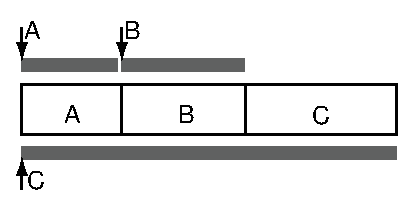
\includegraphics[scale=0.75]{c++-object}
\end{center}
%
The object $A$ is laid out first, followed by $B$, then any additional fields in $C$.  A pointer to
a $C$ object is also a pointer to an $A$, so this coercion has no runtime cost.  The coercion from
$C$ to $B$ is also allowed with a bit of pointer arithmetic.

In OCaml, the situation is quite different.  The order of methods and fields in an object doesn't
matter, coercions to arbitrary supertypes are allowed, and coercions never have a runtime cost.  To
help understand how this works, let's build a model of objects using polymorphic variants.

Abstractly, an object is just a thing that reacts to messages that are sent to it---in other words,
it is a function on method names.  Given an object $o$ with method names $m_1, m_2, \ldots, m_n$, the
names are given variant labels \hbox{\lstinline/`L_m1/}, \hbox{\lstinline/`L_m2/}, $\ldots$, \hbox{\lstinline/`L_mn/}.  The
object becomes a pattern match over method labels, and the fields become let-definitions.
Here is a dog object together with the corresponding model.

\begin{center}
\begin{tabular}{c|c}
Object & Model\\
\hline
\begin{minipage}[t]{2.2in}
\begin{ocamllisting}
type dog =
   < eat : unit;
     bark : unit;
     chase : string -> unit
   >

let dog s =
object (self)
   val name = s
   method eat = printf "%s eats\n" name
   method bark = printf "%s barks\n" name
   method chase s =
      self#bark;
      printf "%s chases %s\n" name s
end
\end{ocamllisting}
\end{minipage}
&
\begin{minipage}[t]{2.2in}
\begin{ocamllisting}
! type model_dog =
!    l:[`L_eat | `L_bark | `L_chase] -> 
!       (match l with
!           `L_eat | `L_bark -> unit
!         | `L_chase -> (string -> unit))

let model_dog s =
   let name = s in
   let rec self = function
      `L_eat -> printf "%s eats\n" name
    | `L_bark -> printf "%s barks\n" name
    | `L_chase -> (fun s ->
          self `L_bark;
          printf "%s chases %s\n" name s)
   in
   self
\end{ocamllisting}
\end{minipage}
\end{tabular}
\end{center}
%
The recursive function \hbox{\lstinline/self/} represents the object.  It takes a method label, and returns
the method value.  The type \hbox{\lstinline/model_dog/} can't be defined in OCaml, because it is
a \emph{dependent} type.  Informally it says that a \hbox{\lstinline/model_dog/} is a function that takes a
label \hbox{\lstinline/l/}.  If \hbox{\lstinline/l/} is \hbox{\lstinline/`L_eat/} or \hbox{\lstinline/`L_bark/}, then the result
type is \hbox{\lstinline/unit/}.  If the label is \hbox{\lstinline/`L_chase/}, the result type
is \hbox{\lstinline/string -> unit/}.

\begin{enumerate}
\item Suppose an animal object is defined as follows.

\begin{ocaml}
type animal = < eat : unit >
let animal s = object method eat = printf "%s eats\n" s end
\end{ocaml}
%
Write the model \hbox{\lstinline/model_animal/} for an animal object.

\item
Given a \hbox{\lstinline/model_dog/} $e$, how is a coercion \hbox{\lstinline/($e$ : model_dog :> model_animal)/} implemented?

\item
How is a coercion \hbox{\lstinline/($e$ : dog :> < chase : string -> unit >)/} implemented in the model?
\end{enumerate}
%
Suppose that, instead of representing fields as individual let-definitions, the fields of an object
are collected in a record, with the compiler inserting the appropriate projections.  For example,
here is a revised \hbox{\lstinline/model_dog/}.

\begin{ocaml}
type dog_fields = { name : string }

let model_dog s =
   let rec self fields = function
      `L_eat -> printf "%s eats\n" fields.name
    | `L_bark -> printf "%s barks\n" fields.name
    | `L_chase -> (fun s ->
          self fields `L_bark;
          printf "%s chases %s\n" fields.name s)
   in
   self { name = s }
\end{ocaml}
%
\begin{enumerate}
\item[4.] In this revised version, how is a functional update implemented?
Explain your answer by giving the model for a new method

\begin{ocaml}
method new_dog s = {< name = s >}.
\end{ocaml}

\item[5.]
What is the complexity of method dispatch?  Meaning, given an arbitrary method label, how long does
it take to perform the pattern match?
\end{enumerate}
%
Suppose the pattern match is hoisted out of the object into a separate function \hbox{\lstinline/vtable/}.

\begin{ocaml}
let model_dog s =
   let vtable = function
      `L_eat -> (fun self fields -> printf "%s eats\n" fields.name)
    | `L_bark -> (fun self fields -> printf "%s barks\n" fields.name)
    | `L_chase -> (fun self fields s ->
          self fields `L_bark;
          printf "%s chases %s\n" fields.name s)
   in
   let rec self fields label =
      vtable label self fields
   in
   self { name = s }
\end{ocaml}
%
\begin{enumerate}
\item[6.]  What are the advantages of the separate \hbox{\lstinline/vtable/}?  What are some disadvantages?
\end{enumerate}

\begin{answer}\ifanswers
\begin{enumerate}
\item 

\begin{ocaml}
let animal_model s =
   let rec self = function
      `L_eat -> printf "%s eats\n" s
   in
   self
\end{ocaml}

\item

A \hbox{\lstinline/model_dog/} has all the methods of a \hbox{\lstinline/model_animal/} so it can be used as an
animal unchanged.  The coercion returns the dog without change.  To be more precise, consider the
types.

\begin{ocaml}
type model_dog = l:[`L_eat | `L_bark | `L_chase] -> $\cdots$
type model_animal = l:[`L_eat] -> $\cdots$
\end{ocaml}
%
The relation \hbox{\lstinline/model_dog $\subtype$ model_animal/} holds because
\hbox{\lstinline/[`L_eat] $\subtype$ [`L_eat | `L_bark | `L_chase]/}.

\item 

A \hbox{\lstinline/model_dog/} can be used as a model-\hbox{\lstinline/< chase : string -> unit>/} without change.

\item

A functional update becomes a record update.
The new method \hbox{\lstinline/new_dog/} is modeled as follows.

\begin{ocaml}
let model_dog s =
   let rec self fields = function
      $\cdots$
    | `L_new_dog s ->
        self { fields with name = s }
   in
   self { name = s }
\end{ocaml}

\item

The pattern match is really just a table lookup, so it can be implemented in $O(\log n)$ time, where
$n$ is the number of labels.  However, the number of labels in the program is fixed, so the pattern
match can be implemented in constant time.

\item

The advantage of hoisting the \hbox{\lstinline/vtable/} is that it can be shared by multiple dog objects.
The disadvantage is that it may be slightly more expensive because of the extra function call.
\end{enumerate}
\fi\end{answer}      
\end{exercise}

% -*-
% Local Variables:
% Mode: LaTeX
% fill-column: 100
% TeX-master: "paper"
% TeX-command-default: "LaTeX/dvips Interactive"
% End:
% -*-
% vim:tw=100:fo=tcq:
